%============================ Project Managenent Document ================================
% define document class
\documentclass[
	a4paper               % paper format
%	,10.5pt               % fontsize
%	,BCOR=18mm            % Binding correction
	,bibliography=totoc   % If enabled add bibliography to TOC
	,listof=totoc         % If enabled add lists to TOC
%	,bilingual
	,monolingual
]{bfhthesis}              % KOMA-script report

\usepackage[
	hidelinks,
	pdfusetitle,
]{hyperref}
\usepackage{tikzducks}
\usepackage{amsmath}

\begin{document}

\frontmatter

\title{Bachelor's Thesis}
\subtitle{Extended BBS?: Management Document}
\author{Joël Gabriel Robles Gasser}
\institution{Bern University of Applied Sciences}
\department{Engineering and Computer Science}
\institute{Computer Science}
\version{0.1}
\advisor{Prof. Dr. Annett Laube \and Prof. Dr. Reto Koenig}
\expert{Dr. Andreas Spichiger}
\degreeprogram{Bachelor of Science in Computer Science}

%----------------  BFH tile page   -----------------------------------------
\maketitle

\addchap{Abstract}
Here an abstract might be placed.


%------------ TABLEOFCONTENTS ----------------
\tableofcontents

%------------ START MAIN PART ----------------
\mainmatter

\chapter{Introduction}

\chapter{Goals}

\chapter{Recap of BLS12-381, BBS and Pairings}
This chapter contains a quick recap about BBS and BLS12-381.
The Mathematics of these topics are out of scope for this Thesis, so only the top level ideas will be discussed.

\section{BLS12-381}
\begin{figure}[h]
    \centering
	\includegraphics[width=4cm]{example-image-duck}
	\caption{The BLS12-381 curve}
	\label{fig:bls12381}
\end{figure}
The Barreto-Lynn-Scott Curves \cite{pairing-friendly-curves} are a group of pairing friendly curves. 
Specifically the BLS12-381 Curve is used in the BBS Signature Scheme \cite{bbs-signature-scheme}.
The 12 in the name comes from the embedding degree, the 381 is the amount of bits necessary to represent a point on the curve.
This Curve is defined as with the following equation $y^2 = x^3 + 4$, where x and y are coordinates on the Field $F_p$.

\subsection{Field Extensions}
$G_1$ is the largest is the largest prime order subgroup of the BLS curve.
For the Pairings discussed in section \ref{sec:pairing} we need multiple points on curves as inputs.
Besides a point on $G_1$ we also need a point on $G_2$.
This $G_2$ is an Extension of the Field $F_p$ into the Field $F_{p^2}$.
This alters the curve equation a bit to $y^2 = x^3 + 4(u + 1)$ where x and y are no longer coordinates but are polynoms of the second order.
Both $G_1$ and $G_2$ are additive Groups.
For the Pairings we also need a third Group, this time in the Field $F_{p^{12}}$.
This is Group is a multiplicative group called $G_T$ in section \ref{sec:pairing}, where x and y are polynoms of the $12^{th}$ order.
With this we now know all the necessary groups for \ref{sec:bbs}.
The Basepoints (generators) of both $G_1$ and $G_2$ are defined in \cite{pairing-friendly-curves} as follows (Big-endian order encoded as HEX):\newline

\boldmath$G_1$(BP1):\newline
x = 0x17f1d3a73197d7942695638c4fa9ac0fc3688c4f9774b905a14e3a3f171bac586c55e83ff97a1aeffb3af00adb22c6bb
y = 0x08b3f481e3aaa0f1a09e30ed741d8ae4fcf5e095d5d00af600db18cb2c04b3edd03cc744a2888ae40caa232946c5e7e1\newline\newline
\boldmath$G_2$(BP2):\newline
$x_O$ = 0x024aa2b2f08f0a91260805272dc51051c6e47ad4fa403b02b4510b647ae3d1770bac0326a805bbefd48056c8c121bdb8
$x_1$ = 0x13e02b6052719f607dacd3a088274f65596bd0d09920b61ab5da61bbdc7f5049334cf11213945d57e5ac7d055d042b7e
$y_O$ = 0x0ce5d527727d6e118cc9cdc6da2e351aadfd9baa8cbdd3a76d429a695160d12c923ac9cc3baca289e193548608b82801
$y_1$ = 0x0606c4a02ea734cc32acd2b02bc28b99cb3e287e85a763af267492ab572e99ab3f370d275cec1da1aaa9075ff05f79be

\section{BBS}
\label{sec:bbs}
\begin{figure}[h]
    \centering
	\includegraphics[width=4cm]{example-image-duck}
	\caption{The Actors of BBS and their connection}
	\label{fig:bbstriangle}
\end{figure}
The BBS Signature Scheme \cite{bbs-signature-scheme} is a multi-message signature scheme with support for selective disclosure and proof of knowledge of the signature, thus proving unlinkability between different verfiers. 
Figure \ref{fig:bbstriangle} shows the flows between the different actors.
For this thesis we define following names for the actors:
\begin{itemize}
	\item Issuer - Issues a signature on a set of messages
	\item Holder - Holds the set of messages as well as the signature. Also generates the Proof for the verifier.
	\item Verifier - Gets the disclosed messages as well as the proof, which he then verifies
\end{itemize}
For the key generation a random scalar \textbf{SK} and the Base Point of $G_2$ are needed.
Thus the public key (calculated as $SK*BP2$) results in Point on $G_2$.
This allows for all other calculations (like the signature or the proof) to be done in $G_1$ which in turn makes the algorithm more efficient.


\section{Pairings}
\label{sec:pairing}
For the verification of the BBS signature and proof Pairing-functions are used. The most important part of these functions are their billiniarity i.e.,\newline
\begin{equation}
		e(A, B + B') = e(A, B)e(A, B') \text{and} e(a * A, b * B) = e(A, B)^{ab}
\end{equation}

With these characteristics we can understand the equations for verifying the signature and proof.\newline

\textbf{Example 1. BBS Signature verification}
\begin{equation}
	\begin{split}
		Identity_{GT} & = e(A, W + BP2 * e) * e(B, -BP2) \\
		& = e(A, BP2 * e)e(A, W)e(B, BP2)^{-1} \\
		& = e(A, BP2)^ee(A, SK * BP2)e(B, BP2)^{-1} \\
		& = e(A, BP2)^ee(A, BP2)^{SK}e(B, BP2)^{-1} \\
		& = e(A, BP2)^{e + SK}e(B, BP2)^{-1} \\
		& = e(B * \frac{1}{sk * e}, BP2)^{e + SK}e(B, BP2)^{-1} \\
		& = e(B, BP2)^{\frac{e + SK}{e + SK}}e(B, BP2)^{-1} \\
		& = e(B, BP2)^1e(B, BP2)^{-1} \\
		& = e(B, BP2)^0 \\
		& = 1
	\end{split}
\end{equation}

\chapter{Use Cases}
For this Thesis we will use a small collection of use cases to demonstrate how BBS should work in conjunction with extensions (like VC's, Link Secrets etc.).

\section{Simply buying a train and mobile subscription}
Lets assume you want to go and buy a train subscription.
Once at the counter, the employee ask you for your ID card, to verify your identity and to get the required data for the subscription.
Now the employee should only need to check if the ID is valid, if the photo on it matches you, something to link your subscription to you (your name is used for that most of the time) and maybe he also needs your birthday for an age specific discount.
By handing out your ID, you lose the ability to selectively disclose information about yourself, and with that you lose your anonymity.


\begin{figure}[h]
	\begin{minipage}{0.28\textwidth}
		\textbf{Client}\newline\newline
		
\begin{tikzpicture}
			\duck[graduate]
		\end{tikzpicture}
	\end{minipage}\hfill
	\begin{minipage}{0.28\textwidth}
		$$\underrightarrow{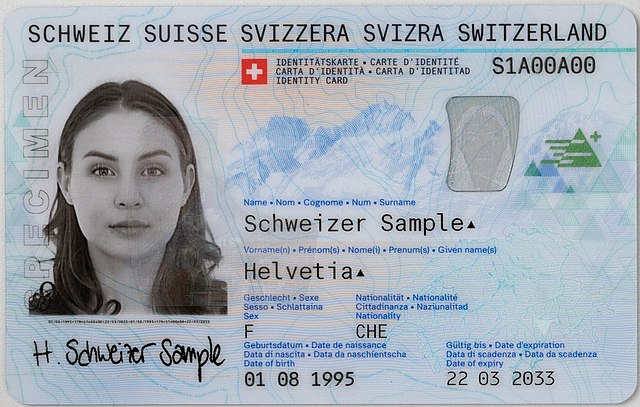
\includegraphics[width=30mm]{./img/ID.jpg}}$$
		$$\overleftarrow{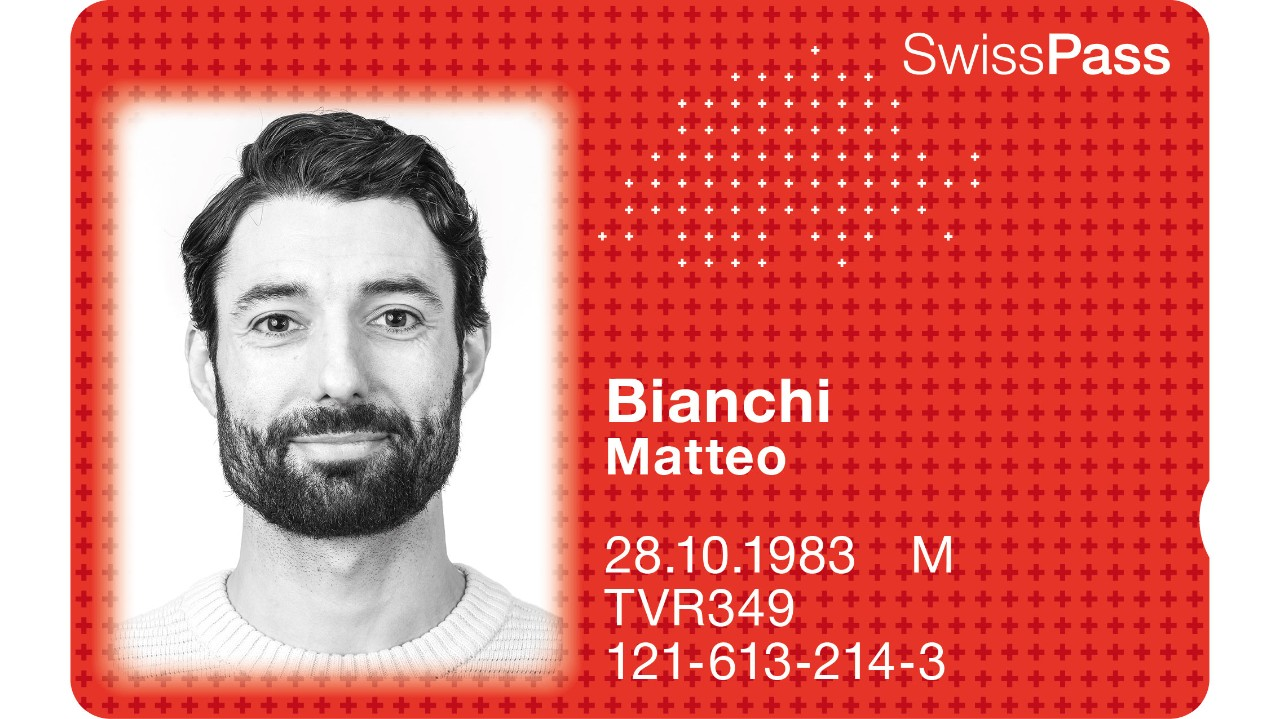
\includegraphics[width=30mm]{./img/Swisspass.jpeg}}$$
	\end{minipage}\hfil
	\begin{minipage}{0.28\textwidth}
		\textbf{SBB}\newline\newline
		
\begin{tikzpicture}
			\duck[tshirt, jacket=blue!50!black, tie=red]
		\end{tikzpicture}
	\end{minipage}
	\caption{Buying a train subscription}
	\label{fig:trainssub}
\end{figure}

Now you also need a mobile subscription. You go to your next Swiss Post office 

 
	





\chapter{Extensions of BBS}

\section{BBS with VC's}
The BBS signatures and proofs as well as the messages need to be transported somehow.
For this Thesis we chose Verifiable credentials \cite{verifiable-credentials} as the representation of these attributes.
But what are VC's? \newline
Verifiable credentials are JSON-LD data models, designed to represent different types of digital credentials.
The Idea, is to be able to translate physical credentials, like an ID or a driver's license, into the digital world.
In this Thesis we will only look at a small part of the standard, just enough that we can use it together with BBS.

\subsection{Prepare VC's for BBS}





\appendix

\chapter{First appendix Chapter}



\bibliographystyle{plain}
\bibliography{refs}

\end{document}
